% !TEX encoding = UTF-8 Unicode

\chapter{Introduction} 
\label{introduction}
\minitoc

\section{Contexte}
\subsection{Histoire de l'épidémiologie}
%L'\ep est dérivée par des observations de la période Hypocrate il y a plus de 2000 ans, suggérant que les facteurs environnementaux affectent l'apparition des maladies. 
L'\ep est une domaine de rechercher qui existe depuis très longtemps. On a trouvé les informations sur les maladies infectieuses comme : la variole, la peste, la lèpre,... dans les anciennes documents du Chine, Inde, Égypte, Rome et Grèce. Dans cette période, les gens a connu que la maladie peut être transmise par les patients aux personnes en bonne santé par le contact avec les patients ou leurs objects personnels. La définition sur l'immunité est aussi formé pendant cette période. L'historien grec Fubidiv (460 - 400 B.C) a découvert que les gens qui sont déjà eu la peste n'auront reçu plus la peste. Alors, ils ont utilisé les personnes qui avaient déjà guéri avec la peste pour soigner celui qui avaient cette malade. En Chine, les gens ont mis des croûte sèche d'un bouton des petite variole dans le nez des enfants pour causer une maladie bénigne, puis créer des anticorps pour lutter contre le variole. Dans la féodalité au Moyen-Âge, la définition sur les maladies contagieuse sont formés lorsque les gens ont réalisé que le contact avec les object personnel, l'air, l'eau ou le nourriture des malades doit contribuer à la transmission des maladies entre les patients et les personnes en bonne santé. 

Jusqu'au $XIX^{\`e}$ siècle, les mesures à grande échelle  sur la distribution des maladies dans les grandes groupes de population sont premièrement effectué en Europe. Typiquement est la découverte de John Snow sur le risque de choléra dans la ville de Londres est lié à la consommation de différentes entreprises\cite{snow1855}. John Snow a trouvé une association claire entre la source d'eau et ces décès en identifiant les locations de chacun des décès de choléra à Londres entre 1848 -1849 et 1853 - 1854. Il a comparé les décès des comtés avec différentes sources d'eau et a montré que la mortalité dans les comtés où l'entreprise Southwark est l'approvisionnement en eau, était plus élevés que dans d'autre comtés. Grâce aux leurs résultats méticuleux, Snow a développé une théorie de la transmission des maladies infectieuses et suggère que le choléra se propage à travers l'eau contaminée.Ses recherches ont eu un impact direct et durable sur la politique de santé publique. 

En 1861, Ignace Philippe Semmelweis, une des premiers médecins qui utilise les statistiques en médecin pour tester une hypothèse sur une étiologie d'une malade, a été publié son travail dans un livre. Il proposait à ses contemporains de se laver les main dans une solution d'hypochlorite (de l'eau de javel) et stérilisait ses instruments de chirurgie. Malheureusement, l'opposition parmi ses contemporains ne permit pas de faire avancer ses idées.
%Cependant, les mesures à grande échelle sur la distribution des maladies dans les grandes groupes de population sont premièrement effectués au $XIX^{\`e}$ siècle. Cette étape marque non seulement le début formel de l'\ep masi aussi les réalisations les plus impressionnantes de cette spécialité\cite{beaglehole2004}. Un exemple très bien connu est la découverte de John Snow sur le risque de choléra dans la ville de Londres est lié à la consommation de différentes entreprises\cite{snow1855}. John Snow a identifié les locations de chacun des décès de choléra à Londres entre 1848 -1849 et 1853 - 1854 et a trouvé une association claire entre la source d'eau et ces décès. Il a comparé les décès des comtés avec différentes sources d'eau et a montré que la mortalité dans les comtés où l'entreprise Southwark est l'approvisionnement en eau, était plus élevés que dans d'autre comptés. Sur la base de ses recherches méticuleuses, Snow a développé une théorie de la transmission des maladies infectieuses et suggère que le choléra se propage à travers l'eau contaminée. Il a encouragé l'amélioration de la qualité de l'eau pendant longtemps avant de trouver des bactéries cholériques. Ses recherches ont eu un impact direct et durable sur la politique de santé publique. 
À la fin du $XIX^{\`e}$ siècle et au début du $XX^{\`e}$ siècle, des méthodes mathématiques furent introduit en \ep par Ronal Ross, W.O Kermarck et A.G McKendrick \cite{kermack1927},\cite{kermack1932},\cite{kermack1933}. Cette approche a été initialement appliqué à la lutte contre les maladies infectieuses et s'est avérée efficace pour mettre en évidence une association entre certaines conditions ou agents environnementaux à des maladies déterminée. Dans la deuxième moitié du $XX^{\`e}$ siècle, en particulier dans les pays à revenue élevé ou moyen, cette méthode est applicable aux maladies non transmissible chronique telles que les maladies cardiaques et le cancer. 

Avec l'apparition des maladies nosocomiales, d'une antibiorésistance préoccupant, des circulations rapidement des microbes sur notre planète, La veille écoépidémiologique et l'accès rapide à des information transparentes et valides devient majeur problème. Un des publication très célèbre au début du deuxième moitié du $XX^{\`e}$ siècle est la recherche de Richard Doll et Andrew Hill sur la relation entre tabagisme et le cancer du poumon\cite{doll1964}. Ils ont effectué des observation sur 41,000 homme et femme au Royaume-Uni avec des condition médicale qualifié pendant 12 ans. Ils ont montré que la mortalité par le cancer du poumon a fortement augmenté chez les fumeurs pendant des années 1952 - 1961. Le taux de mortalité par cancer du poumon est plus élevé chez les légers et moyen fumeurs qui inhalent que chez ceux qui n'inhalent pas.

Le tabagisme est un cas particulier dans l'\ep, mais pour la plupart des maladies, il existe plusieurs facteurs qui contribuent à la cause. Le travail de recherche pour identifier la relations entre les maladies et les facteurs causal devient une grande problème dans la domaine l'\ep. De nouvelle méthodes épidémiologiques sont utilisées pour analyser ces relations. L'\ep joue un rôle très important dans la détection et le contrôle des maladies dans des pays à revenue faible ou intermédiaire comme le VIH / SIDA, la tuberculose et le paludisme. Cette branche d'épidémie devient de plus en plus important dans tous les pays du fait de l'émergence de nouvelles maladies transmissibles comme le syndrome respiratoire aigu sévère (SRAS), l’encéphalopathie spongiforme bovine (ESB) et la grippe pandémique. L'\ep a considérablement évolué ces 50 dernières années et son principal défi à l’heure actuelle consiste à explorer et à agir sur les déterminants sociaux de la santé et de la maladie, dont la plupart se trouvent en dehors du secteur sanitaire.

\subsection{Portée, applications et difficultées de l'\ep }
\subsubsection{Portée}

L'\ep est une science théorique fondamentale de la médecine et des autres autres science de la santé. Elle est largement utilisée dans la recherche et les services de santé publique quotidiens. L'\ep s'intéresse sur la relation entre la santé humaine et les facteurs environnementaux (géographiques, biologiques, sociaux, etc...). Cette relation peut avoir un effet positif ou négatif sur la santé de la communauté. Le but de l'\ep est de l'analyse et de la comprendre afin de fournir des meilleurs interventions au bénéfice de la communauté.

\subsubsection{Applications}
\begin {itemize}
	\item{Cause de la maladie : l'\ep découvre les causes des maladies. La majorité des maladies sont causées par les interactions entres les facteurs génétiques et environnementaux (Figure \ref{Pic1}).
\begin{figure}[h]
%\begin{center}
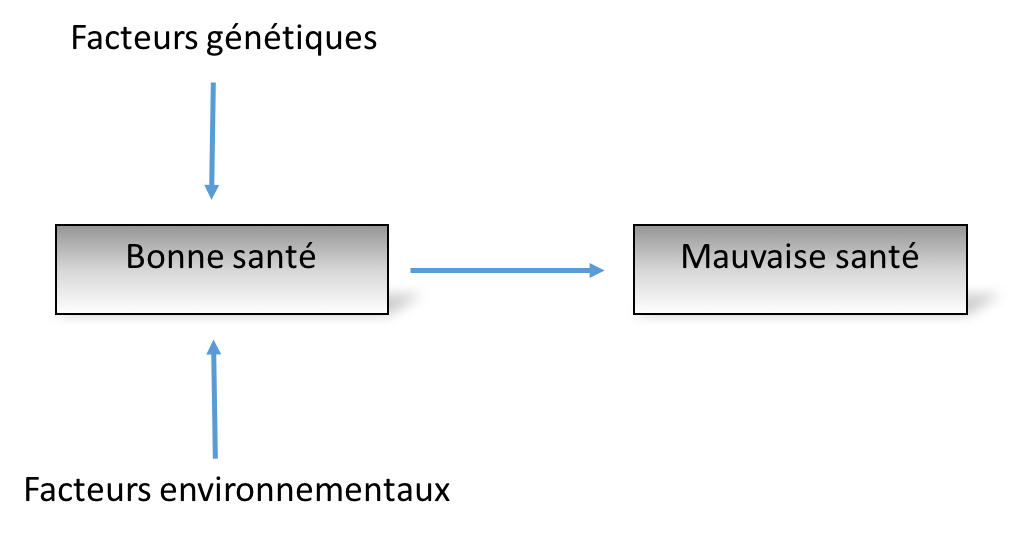
\includegraphics[width = \linewidth]{../figures/chap1/Pic1.png}
\caption{Cause}
\label{Pic1}	
%\end{center}
\end{figure}
}

\item{Histoire naturelle de la maladie : L'\ep aussi s'intéresse sur l'évolution et l'histoire naturelle des maladies chez les individus et les groupes (Figure \ref{Pic2})
\begin{figure}[h]
%\begin{center}
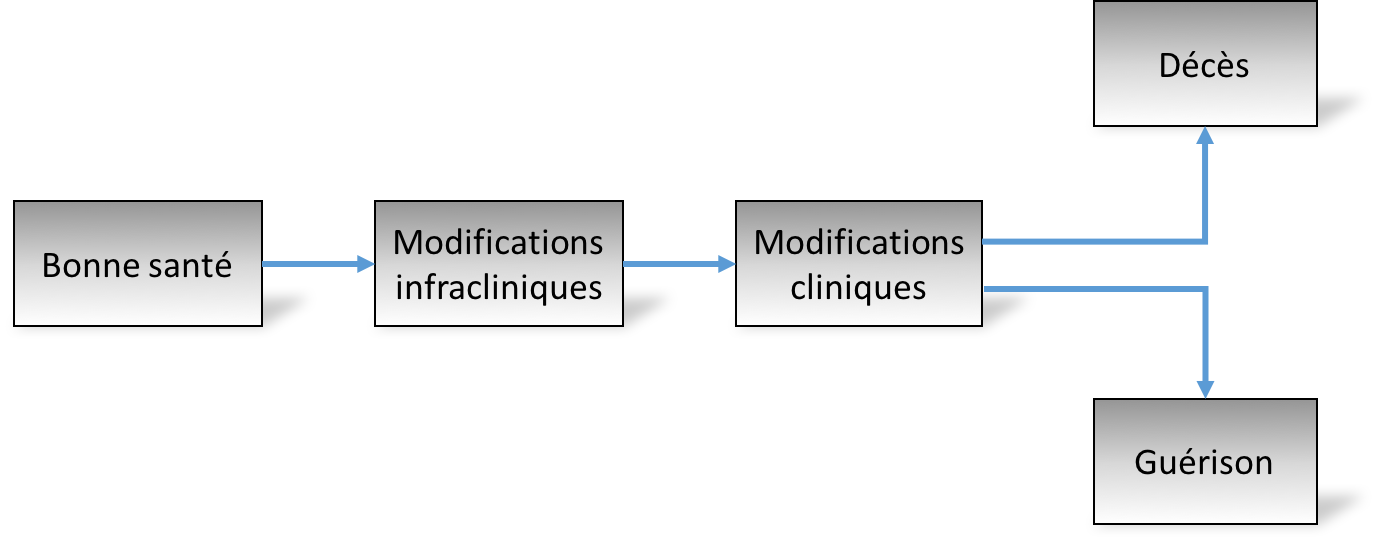
\includegraphics[width = \linewidth]{../figures/chap1/Pic2.png}
\caption{Histoire naturelle}
\label{Pic2}	
%\end{center}
\end{figure}
}

\item{Situation sanitaire des populations : L'\ep est souvent utilisée pour décrire état de santé des groupes de population (Figure \ref{Pic3}). 
\begin{figure}[h]
%\begin{center}
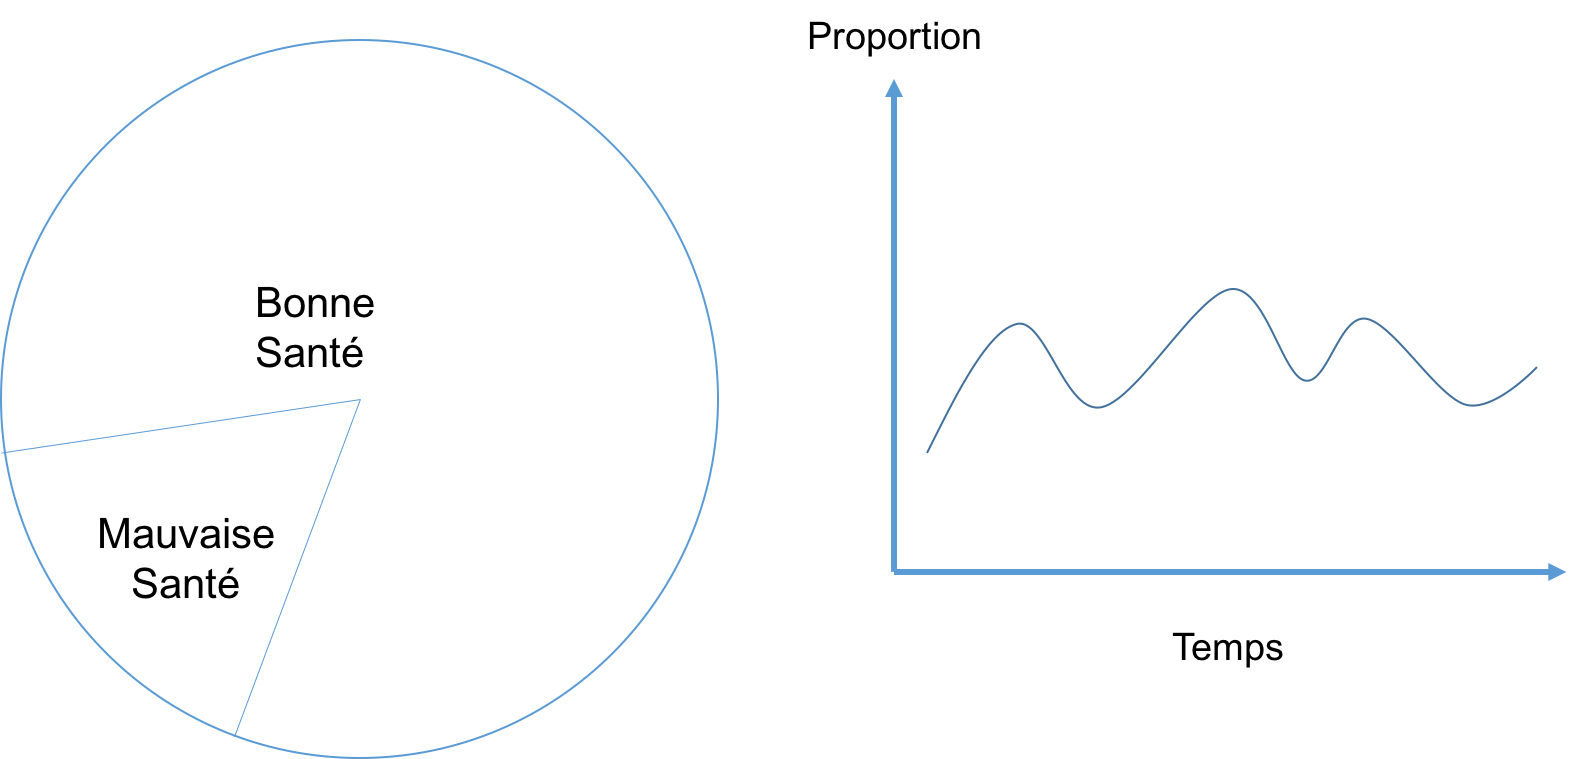
\includegraphics[width = \linewidth]{../figures/chap1/Pic3.png}
\caption{Description de l'état de santé des populations}
\label{Pic3}	
%\end{center}
\end{figure}
}

\item{Évaluation des interventions : l'\ep est utilisée pour évaluer l'efficacité des services de santé (Figure \ref{Pic4}). L'application des principes et méthodes épidémiologiques aux problème rencontrés dans la domaine médical a conduit à la développement des autres domaines comme l'\ep moléculaire, l'\ep génétique, le pharmaco-\ep,.... 
\begin{figure}[h]
%\begin{center}
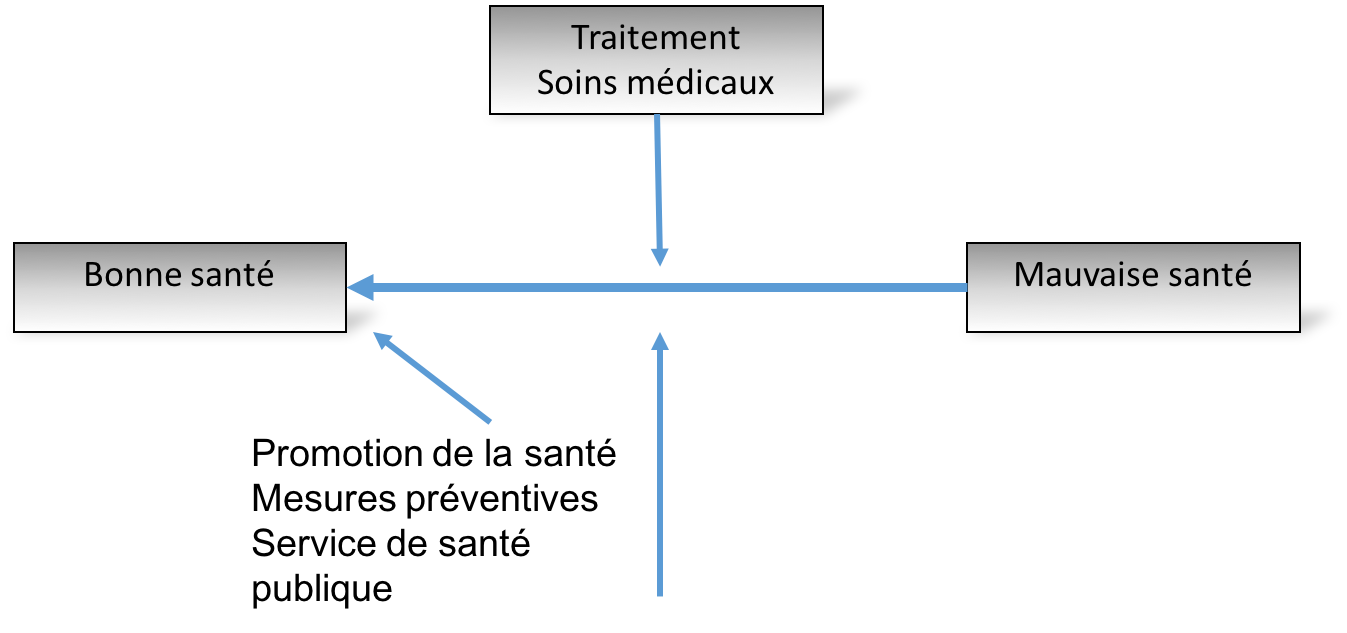
\includegraphics[width = \linewidth]{../figures/chap1/Pic4.png}
\caption{Évaluation des interventions}
\label{Pic4}	
%\end{center}
\end{figure}
}
\end{itemize}

\subsubsection{Difficultées}
Sous l'impact du changement climatique et de la pollution de l'environnement, de nombreuses nouvelles maladies infectieuses apparaissent et causent de grands dommages à la santé public comme le SARS, l'Ebola, le Zika, le grippe pandemique (H5N1, H7N9, H1N1, H5N6 ),... L'\ep doit continuellement traiter les problèmes découlant de ces nouvelles infectieuse maladies et fournir des interventions opportunes pour limiter leurs propagation au sanitaire des populations. 

Une autre limite de l'\ep est la contradiction entre les résultats des recherche de l'\ep. Par exemple, en Janvier 1994, une étude en Suisse a révélé une association statistiquement significative entre l'exposition au radon et le cancer du poumon, contrairement à l'étude menée au Canada. Dans le même temps en Janvier 1994, un étude sur les électriciens américains a révélé qu'il peut y avoir un lien entre des champs électromagnétiques dans les fils électriques et le cancer au cerveau. Cependant, une étude précédente en 1993 en France et au Canada a montré qu'il n'y avait pas d'association entre le champ électromagnétique et la leucémie. Les contradictions dans les résultats de recherche ont causé la confusion sur la population et cela a affecté négativement sur le succès des campagnes prophylactique de l'\ep.

\subsection{Les réalisations de l'épidémiologie}
\subsubsection{Tubercolose}
Plus de 1 milliard de personnes sont mortes de la tuberculose depuis 200 ans et le nombre de cas de tuberculose est devenu la maladie infectieuse la plus meurtrière de l'histoire de l'humanité. Avec la prévalence de la tuberculose, cette malade est présente dans tous les pays. Cependant, la tuberculose affecte beaucoup les pays en cours de développement, où la maladie n'est pas bien contrôlée et le taux d'inflection est élevé.

En fait, l'incidence de la tuberculose et leurs décès a diminué régulièrement depuis les années 1900. Avant que l'homme a trouvé le spécifique contre la tuberculose, l'amélioration de l'hygiène, du logement et de la vaccination ont entraîner une réduction des taux d'infection dans certains pays. Mais seulement lorsque les antibiotiques sont nés, la tuberculose devient une maladies qui peut être contrôlée et guérie. Sans antibiotiques, jusqu'au 70\% des patient tuberculose seront morts. Le vaccin antituberculeuse a été existé depuis un siècle. Mais il ne se révèle efficace que dans la prévention de la tuberculose chez les enfants. Les vaccin antituberculeuse ne sont pas efficaces lorsqu'il sont utilisés avec les adultes.

En général, la tuberculose est toujours sous contrôle avec les progrès du traitement. Cependant, la tuberculose est encore assez complexe dans certains pays en développement. Des ressources financières et politique seront nécessaires pour soutenir le contrôle de la tuberculose.
\subsubsection{VIH/AIDS}

Au début des années 1980, aux États-Unis, certains hommes gais ont eu une infection anormale. Dans les années suivantes, la maladie est devenue de plus en plus commune. Les chercheurs ont finalement découvert un virus qui causait l'immuno-déficience chez eux. C'est le VIH - un virus originaire d'Afrique qui infecté uniquement par des primates. Dans 100 dernières années, le VIH a commencé à infecter les humaines et s'est rapidement propagé dans le monde entier. 

Le VIH se propage dans le sang, principalement par des activités sexuelles non sécuritaires, de transfusions sanguines provenant de sources infectées, de partage d'aiguilles, de la mère à l'enfant pendant la grossesse, l'accouchement ou l'allaitement.

Une personne infectée par le VIH non traitée doit devenir le SIDA, également connu sous le nom de syndrome d'immuno-déficience acquise. La maladie détruit le système immunitaire humain, offrant des possibilités d'infections opportunistes et causant la mort.

Il n'y a pas de vaccins disponibles pour prévenir l'infection par le VIH, et aucun traitement ne peut éliminer complètement le virus du VIH de l'organisme.Cependant, les personnes vivant avec le SIDA peuvent maintenant étendre et améliorer leur qualité de vie grâce à la thérapie anti-rétrovirale (ART). ART est la thérapie qui utilise des médicaments anti-rétroviraux, qui ralentissent la réplication du VIH dans le corps. Par conséquent, le traitement anti-rétroviral augmentera l'immunité et réduira les risques d'infections opportunistes chez les patients infectés par le VIH.

Actuellement, les scientifiques travaillent toujours pour trouver un remède et arrêter le VIH / SIDA. Ils espèreront
d'arrêter cette pandémie au 2030.

\subsubsection{Variole}
La variole ou petite vérole est une maladie infectieuse d'origine virale, très contagieuse et épidémique, due à un poxvirus. Il est apparu chez les humains depuis des millénaires et devient un facteur majeur dans l'histoire de l'humanité. À la fin des années 1960, la variole était encore complexe en Asie et en Afrique, avec environ 2 millions de décès chaque année.

La variole se propage facilement entre les gens, par les éternuements ou les contacts occasionnels. Il provoque des symptômes simples avec des pustules sur la peau, et peut entraîner des complications causée par les nombreuses cicatrices comme l'arthrite, la cécité, la mort... Au $XVIII^{\`e}$ siècle, un médecin britannique, Edward Jenner, a découvert que les vaches pouvaient également être infectées par le virus de la variole. Les personnes qui sont infectées par le virus de la variole chez les vaches peuvent facilement être guérie et ils sont également immunisées contre la variole humaine. Jenner devina que c'était une type de virus variola plus légère. Il a extrait les croûte d'un bouton d'une personne qui a été infecté par la variole chez les vaches et les a injectées dans les bras d'un garçon de huit ans. Étonnamment, ce garçon était immunisé contre la maladie. Jenner est devenu l'invention de la vaccination et aussi le créateur du vaccin contre la variole.

Grâce à la méthode vaccination de Jenner, l'homme a trouvé et développé des méthode de prévention de la variole à l'échelle mondiale. Les campagnes de vaccination sont poursuivies du $XIX^{\`e}$ siècle au $XX^{\`e}$ siècle. Jusqu'au 8 Mai 1980, l'éradication de la variole a été proclamée par l'Organisation Mondiale de la Santé (OMS).


\subsubsection{Grippe}
Au cours des derniers siècles, la grippe a également causé plus de décès que le VIH/AIDS. Les pandémies saisonnières de grippe se produisent chaque année et touchent environ quatre millions de personnes, avec environ 250 000 décès dans le monde entier. Au cours du dernière siècle, il y avait des nouveaux type du virus de la grippe sont propagée à l'homme à partir de la volaille ou du bétail comme les grippes H1N1, H5N1, H5N6, H7N9,.... Ces types de virus sont complètement nouvelles et ils créent des pandémies dévastatrice lorsqu'ils commencent à se propager entre les hommes. 

Un exemple typique est la pandémie de la grippe A/H1N1 en 1918, également connue sous le nom de grippe espagnol, qui a causée la mort de plus 50 - 100 million de personnes, soit 2 - 5 fois plus grande que le nombre des victimes de la premier guère mondiale. 

De nos jours, l'épidémie de grippe a lieu partout dans le monde. Selon l'OMS, cette maladie survient chaque année, entraînant la situation entre 3 millions et 5 millions de personnes atteintes de la grippe sévère et environ 250 000 à 500 000 décès chaque année dans le monde. Il n'existe pas encore les vaccins qui peut lutter contre la variation des nouveaux type de virus de la grippe. C'est pourquoi l'OMS a donnée des notification en haut niveau qui appelant les pays à surveiller la situation de la grippe afin de réduire la possibilité d'explosion d'une épidémie de grippe pandémique en échelle mondiale. 

Les quatre maladies ci-dessus sont des maladies transmissible plus typique dans des 100 derniers années. En fait, il existe des autres maladies peuvent également figurer sur cette liste, notamment la poliomyélite, le paludisme, le choléra et la syphilis.

\subsection{Dengue}
La dengue est une infection virale qui endémique dans les pays tropicaux. Elle transmise entre les être humain par l'intermédiaire des moustique. Cette infection virale entraîne classiquement fièvre, maux de tête, douleurs musculaires et articulaires, fatigue, nausées, vomissements et éruptions cutanées.  La guérison survient généralement en une semaine.  À côté des symptômes cités là, Il existe des formes hémorragiques ou avec syndrome de choc, rares et sévères, pouvant entraîner la mort.

Dans le passé, les africains sont utilisé le mot Ka-dinga pepo pour appeler la maladie dengue qui transmise par les moustique Aedes Aegypti. En Swahili, cet mot signifie "malade du diable" parce ce qu'elle créer le bouleversement et la débilité de l'intérieur le corps des victimes qui mener l'hémorragie des organes internes. La maladie Ka-dinga pepo n'a été apparu que dans les régions tropicales et subtropicales. Au cours des siècle, cette maladie a été propagée partout dans le monde entier à cause de la développement de la circulation et de la commerce. Jusqu'au $XVIII^{\`e}$ siècle, en 1780, elle a causé une pandémie sur la province Philadenphia d'Amérique. 

Au dernier du $XX^{\`e}$ et début du $XXI^{\`e}$siècle, la dengue est devenu une menace très dangereux avec la vitesse de propagation très horrible dans le monde entier, même aux États-Unis avec le système sanitaire le plus énergique. Le taux de propagation de la dengue est devenu très sérieux ces dernières années. Avant 1970, il y avait que 9 pays qui sont touché par cette malade mais cette nombre a été quadruplé en 1995. Selon l'Organisation mondiale de la santé (OMS, 2007), environ 40\% de la population mondiale dans 112 pays du monde est exposée au virus. On estime à 390 millions le nombre de nouvelles infections chaque année\cite{bhatt2013}.

Afin de prévenir la maladie, les premiers vaccins développés par des scientifiques japonais et américains après l'identification du virus. La problème principal est que la dengue a non seulement un mais 4 type de virus : Dengue 1, Dengue 2, Dengue 3, Dengue 4. Une zone peut être infecter par un, deux ou plusieurs types de virus en même temps.  De plus, ces types de virus se muent souvent très rapidement, rendant le système immunitaire humain difficile à résister. Avec la plupart des types de virus, les personnes qui sont déjà infectent par une malades ont souvent des anticorps qui aident le corps à la résistance lors d'infections ultérieures. Les vaccins sont construits sur le même mécanisme. Cependant, en raison de la complexité du virus, les personnes atteintes d'anticorps Dengue 1 peuvent  toucher aux trois autres types de virus Dengue. 

Avec le développement de la technologie moderne, les scientifiques ont obtenu quelques succès dans l'étude des vaccins contre la dengue. Dans la deuxième guerre mondiale, les scientifiques avait utilisée Dichloro-Diphényl-Trichloréthane (DDT) pour exterminer les moustiques. Cela a contribué à arrêter la fièvre dengue et malaria au centre et au sud d'Amérique. Pourtant, depuis la fin des années 1960, le DDT a été abandonné en raison de problèmes sanitaires et environnementaux. Ceci est entraîné le retour des moustiques et leurs maladies infectieuses. Récemment, le Dengvaxia dengue vaccine a été distribué au Mexique, au Brésil, au Salvador et aux Philippines. Cependant, leurs efficacité ne sont pas élevée car ils existe des inconvénient et le coût sont très élevée. Jusqu'à maintenant, le monde n'a pas encore trouvé un bon et efficace vaccin pour cette maladie. C'est la raison pour laquelle les domaines d'\ep ont activées les recherches et les analyses des impacts et des interactions environnementaux sur le vecteur le plus dangereux dans l'histoire humanité. 

\section{L'\'etat de l'art}
Un certain nombre d'études ont cherché à caractériser les influences du climat, de la démographie humaine et du comportement sur l'épidémiologie des maladies infectieuses, en utilisant différentes méthodologies.  Zhang et al. \cite{zhang2008}, Cumming et al. \cite{cummings2009}, Barreto et al. \cite{barreto2008} ont utilisé des modèles mathématiques pour étudier l'effet du changement climatique, de la transition démographique et de la structure urbaine sur la transmission de la dengue. Un résultat global est que les relations quantitatives entre le climat et les maladies à transmission vectorielle sont incohérentes entre les différentes études. Certaines données établissent un lien étroit entre l'incidence de la dengue et El Ni\~{n}o dans les îles du Pacifique \cite{hales1996,hales1999} et en Thaïlande \cite{cazelles2005}, tandis que d'autres constatent que l'augmentation de la densité de population et l'insuffisance des sources d'eau sont les principaux facteurs de l'épidémiologie de la dengue \cite{teixeira2006,gubler2004}. En analysant les données mensuelles de la dengue hémorragique (DHF) en Thaïlande de 1983 à 1997, Cumming et al. \cite{cummings2004} a montré que les zones rurales à faible densité de population peuvent également connaître de graves épidémies.

L'Asie du Sud-Est est une région de circulation dengue particulièrement intense \cite{van2015}, et c'est aussi le cas du Vietnam. Le Vietnam a cette particularité supplémentaire d'avoir une diversité importante de climats sur une zone relativement petite (330 000 km$^2$). Cette diversité climatique est générée par une grande latitude orthogonale à une large gamme d'élévations depuis le niveau de la mer sur la côte Est jusqu'à plus de 3 000 m sur la frontière Ouest. Schmidt et al. \cite{schmidt2011} a réalisé une étude de cohorte et une analyse spatiale au Vietnam et a montré que le risque de dengue était plus élevé dans les zones rurales avec une mauvaise alimentation en eau que dans les zones urbaines à forte densité de population. Do et collaborateurs \cite{hu2013,do2014} ont étudié la dengue dans la ville de Hanoi entre 2004 et 2009 et ont mis en évidence une forte saisonnalité de l'épidémiologie de la dengue avec des incidences élevées entre juin et novembre, saison des pluies qui correspond également à des températures élevées. Le et al. \cite{le2015} a analysé l'influence du tourisme sur l'incidence de la dengue sur l'île de Cat Ba (nord du Vietnam) de septembre à novembre 2013. Ils ont montré que la transmission de la dengue est peu probable sur l'île de Cat Ba. l'introduction de virus de la partie continentale, très probablement Hanoi. Cazelles et ses collaborateurs \cite {thai2010} ont analysé la dynamique de l'incidence de la dengue dans la province de Binh Thuan, au sud du Vietnam. Ils ont utilisé la décomposition en ondelettes pour détecter et quantifier la périodicité de la dengue entre janvier 1994 et juin 2009 et pour décrire le profil de la synchronie dans le temps et l'espace. Ils ont également utilisé cette méthode pour explorer la relation entre l'incidence de la dengue et l'oscillation australe El Ni\~{n}o (ENSO) et ont trouvé une forte association non stationnaire entre les indices ENSO et les variables climatiques pour la période de 2-3 ans.

Ces études ont montré l'influence des facteurs environnementaux sur la transmission de la dengue épidémie. Cependant, ce sont des analyses locales à petites échelles. Il n'existe pas encore une étude à grande échelle permettant d'analyser spécifiquement la relation entres les facteurs environnementaux et la propagation de cette épidémie. 
%En outre, après avoir considéré de nombreux exemples publiés dans le domaine, surtout ceux évoqués dans \cite{keelingsite}, nous avons constaté que les préoccupations de l'épidémiologie ont tendance à se mélanger les unes avec les autres à deux niveaux, celui de la conception (l'étude des flux des individus entre les compartiments) et celui de l'implémentation (par exemple, les EDO du modèle).
%Pour faciliter l'extensibiliité des modèles, il est également souhaitable de pouvoir exprimer certaines préoccupations du domaine de façon séparée. Celles-ci comprennent la distribution de la population étudiée dans des régions spatiales, des intervalles d'âge, sexes, espèces, souches virales\ldots
%Cependant, la séparation des préoccupations en épidémiologie n'est pas aisée car ces préoccupations ne peuvent pas être complètement indépendantes. Par exemple, un concept général de la distribution spatiale de la maladie peut être défini de façon indépendante de celui des espèces d'hôtes. Cependant, certaines espèces hôtes considérées pour la maladie étudiée peuvent être aussi distribuées de façon différente dans l'espace.
%En modélisation épidémiologique, il est essentielle de pouvoir exprimer les hétérogénéités entre individus causées par chacune des préoccupations.
%Il nous faut donc trouver un moyen qui permet de pouvoir définir les préoccupations épidémiologiques de façon séparée tout en permettant de pouvoir exprimer les dépendances dynamiques entre elles.

% et ceux de la simulation (les formalismes déterministe, stochastique ou multi-agents).
%Un grand nombre de travaux en génie logiciel a porté sur les logiciels dont les différents espaces de variation (ou aspects) sont d'une part entremêlés et d'autre part éparpillés dans le code (ou les différents artéfacts) au lieu d'être modulaires c'est-à-dire bien localisés dans des modules (classes, fonctions ...) et séparés les uns des autres. Le fait que les aspects se croisent (\textit{cross-cut}) alors qu'ils devraient pouvoir être compris et en principe devraient pouvoir varier largement indépendamment les uns des autres induit de nombreux défauts : le code est plus difficile à comprendre, à modifier et à réutiliser \cite{HL95soc}\cite{kiczales1996}.
%
%Une préoccupation est un aspect qu'il est difficile de rendre modulaire avec les abstractions classiques de la programmation (fonctions et classes). La séparation des préoccupations vise à surmonter cette difficulté de façon a éviter les défauts que nous venons de citer  \cite{HL95soc}. C'est dans ce cadre que se situe cette thèse, bien que la démarche que nous allons proposer, comme nous le verrons, se démarque très nettement des techniques classiques de séparations des préoccupations qui opèrent typiquement au niveau du code.
%
%Plus précisément cette thèse vise à séparer les aspects épidémiologiques (le premier espace de variation que nous avons identifié) des autres aspects (ceux des deux autres espaces de variation) mais surtout de les séparer les uns des autres. En fait les deux enjeux se rejoignent car pour séparer les aspects épidémiologiques les uns des autres nous les formaliserons ce qui prépare naturellement leur séparation des autres aspects.
%
%Dans la suite de ce document et sauf mention contraire nous appellerons donc
%aspects, ou préoccupations, les aspects épidémiologiques : le statut infectieux
%(SIR ...), la distribution de la population étudiée dans l'espace, selon les
%âges, les sexes, les espèces (hôtes, vecteurs), les souches virales \ldots En
%effet, comme nous le verrons, ces aspects sont typiquement éparpillés et
%entremêlés dans les modèles épidémiologique, y compris dans les modèles
%mathématiques. Dans leurs implémentations, ces aspects sont de plus mêlés aux
%autres espaces de variations que nous avons mentionnés et exprimés dans des
%langages de relativement bas niveau comme MATLAB ce qui exige des compétences en
%programmation. On peut le constater par exemple sur les programmes du site internet de l'ouvrage classique de Keeling et al. "Modeling Infectious Diseases in Humans and Animals" \cite{keelingsite}.
%
%Les techniques classiques de séparation des préoccupations, notamment la programmation par aspects, se situent à niveau d'abstraction trop bas pour pouvoir tirer pleinement profit de la sémantique d'un domaine applicatif particulier comme la modélisation épidémiologique. Nous avons donc adopté un point de vue plus abstrait.
%
%Notre problème principal consistera donc à déterminer si on peut donner une structure aux modèles épidémiologiques. Au minimum on cherchera un opérateur qui soit une loi de composition interne sur l'ensemble des aspects. De préférence on aimerait que l'opérateur soit associatif et commutatif pour ne pas avoir à se préoccuper des parenthèses ni de l'ordre des aspects dans un modèle. Un problème secondaire consistera à séparer l'expression de cette structure des détails d'implémentation.
%
%Une difficulté nous attend : les aspects de la modélisation épidémiologique paraissent a priori difficiles à séparer du statut infectieux. Considérons par exemple un modèle incluant la distribution spatiale de la population dans certaines régions. Si cette distribution était complètement indépendante du statut infectieux des individus, elle n'aurait guère d'intérêt : autant étudier la population dans son ensemble plutôt que de la découper inutilement en régions. Si un modèle inclut un aspect, c'est parce que ce dernier présente, au moins potentiellement, des hétérogénéités par rapport au statut infectieux. C'est donc qu'il y a des interdépendances entre le statut infectieux et cet aspect, ce qui a priori rend difficile leur séparation.

%Pour rendre modulaires les modèles, il nous faut trouver un moyen qui permet de définir des aspects de façon séparée et un opérateur qui permet de combiner ces aspects pour construire des modèles.
%Cet opérateur devrait permet de composer aspects avec aspects ou avec modèles. Du point de vue mathématique, il faut que l'opérateur soit au minimum une loi de composition interne associative \cite{bourbaki1968}, dont la composition des aspects modulaires résulte d'un aspect modulaire et la composition des aspect avec un modèle (qui est une structure composée des aspects modulaires) résulte d'un autre modèle.L'ensemble de modèles et l'opérateur constituent donc un monöide - une structure algébrique. Pour faciliter la réutilisation des parties (aspects modulaires) des modèles et la substitution d'un aspect à un autre, il faut que ce monöide soit commutatif.  Il faut également trouver un moyen pour exprimer des hétérogénéités causées par des aspects épidémiologiques lorsqu'ils se présentent en même temps dans un modèle.

%En outre, l'écriture des modèles en épidémiologie, surtout les modèles complexes qui combinent plusieurs aspects épidémiologiques, est compliquée quand on a peu d'expérience en codage informatique (par exemple, les médecins, les biologistes etc.).
%Pour faciliter l'écriture des modèles, il est important d'avoir à notre disposition un outil de modélisation qui fournit un niveau d'abstraction pour générer efficacement différents types d'implémentation tout en permettant un degré de flexibilité suffisant pour pouvoir exprimer pleinement les différents aspects épidémiologiques que l'on souhaite considérer.
%Autrement dit, il est souhaitable de pouvoir séparer la spécification des modèles de leur simulations (la séparation des préoccupations du domaine de celles de la programmation/simulation) pour que l'on puisse varier l'une de façon indépendante de l'autre. 
%De plus, il est souhaitable également que cet outil permette de pouvoir exprimer des aspects épidémiologiques séparément et les recombiner pour construire des modèles.
%
%Certains outils ont été développé dans le but de faciliter le codage des modèles épidémiologiques. 
%Ils permettent aux utilisateurs de spécifier leurs modèles puis de lancer des simulations afin de pouvoir étudier leur fonctionnement. Par contre, ces outils peuvent s'intéresser à certains sujets spécifiques en épidémiologie (par exemple, FluTE \cite{chao} ou InfluSim \cite{duerr,eichner} visent à étudier la propagation de la grippe, GLEAMviz \cite{balcan, broeck} se focalise sur la transmission spatiale etc.) ou ne permettent que certains types d'implémentation pour la simulation (par exemple, GLEAMviz \cite{balcan, broeck} vise à faire la modélisation stochastique, FRED \cite{grefenstette} permet de formaliser des modèles multi-agents, STEM \cite{falenski, ford} permet de générer des modèles déterministes et stochastiques etc.).

\section{Notre proposition}
Notre premier objectif était d'effectuer un pré-traitement sur les données, puis le visualiser pour avoir un aperçu sur la situation d'épidémie du région Sud-Est d'Asie durant la période 17 ans. Ensuite, nous appliquons les méthodes classification pour grouper la situation d'épidémie des provinces des pays dans la région Sud-Est d'Asie.

Notre prochain objectif est déterminer la relation entre les facteurs environnementaux et la développement de l'épidémie durant la période 1994 au 2010. Plus précisément, les facteurs d'environnementaux sont les facteurs climatiques comme les températures (average, maximal, minimal), l'absolute humidité, la relative humidité, la pluviosité, l'heure de soleils. Parmi les pays dans la région Asie du Sud-Est, nous avons choisi le pays Vietnam où leurs données sont les plus complètes. Nous avons utilisée les méthodes d'analyse ondelette, causalité de Granger et convergence cross mapping pour analyser les relations entre l'incidence de la dengue et les facteurs climatiques sur 64 provinces et 67 station climatique au Vietnam. 

%Notre premier objectif est donc de définir de façon aussi générale que possible l'ensemble des aspects en modélisation épidémiologique et de le structurer. Idéalement les modèles seraient même entièrement composés de ces aspects et du schéma infectieux (SIR ou une de ses variantes). 
%
%%Cette démarche nous semble assez originale en séparation des préoccupations où les contributions sont plus typiquement au niveau du code. Notre parti pris est donc de monter en abstraction de façon à essayer de profiter de la sémantique du domaine et accessoirement de préparer notre deuxième objectif qui est de séparer autant que possible l'expression des modèles des détails d'implémentation.
%
%Nous avons mis de côté les modèles agents, trop complexes, pour nous focaliser
%sur les modèles déterministes et stochastiques en observant que l'on peut
%passer, sous certaines hypothèses d'une représentation à l'autre. Nous nous
%concentrons donc sur les modèles stochastiques, bien qu'ils soient parfois
%exprimés sous forme d'ODE, les hypothèses de stochasticité (distribution de
%Poisson, ...) étant classiques et donc implicites.
%
%Ces modèles peuvent être représentés par des automates stochastiques dont les états sont les
%compartiments et dont les transitions sont étiquetées par les taux (les éléments
%strictement positifs) dans la matrice des taux de transition de la chaîne de Markov.
%Or nous avons constaté que les aspects qui nous intéressent peuvent eux-aussi être représentés par des automates stochastiques.
%
%En cherchant dans la littérature, nous avons trouvé que ces automates avaient justement été dotés, bien que dans un domaine complètement différent, de l'opérateur idéal : un opérateur tensoriel (la somme tensorielle $\oplus$  dans le cas des CTMC) \cite{plateau1991, plateau2000}. Un opérateur tensoriel est idéal parce qu'il donne à l'ensemble des aspects une structure de monoïde.
%
%Nous avons donc pu proposer une définition très générale des aspects et des modèles (des combinaisons d'aspects) en leur donnant les propriétés voulues pour la séparation des préoccupations et ce d'autant plus que l'opérateur tensoriel peut être rendu commutatif.  
%
%Toutefois il nous fallait encore permettre d'introduire des hétérogénéités par rapport au statut infectieux comme nous l'avons souligné plus haut. Nous avons pour cela réutilisé la notion de taux fonctionnel de \cite{plateau2000} qui consiste à permettre à la définition de taux de transition de dépendre de l'ensemble des états de l'automate. Le point à souligner est que les modèles proprement dits, c'est-à-dire la définition des aspects et leur composition, ne sont pas concernés par ces dépendances induites par le taux fonctionnel qui sont différées à une phase d'instanciation.
%
%%Nous avons même élargi encore la notion d'aspect épidémiologique en identifiant les aspects aux morphismes de l'ensemble des modèles. En particulier, au lieu de dire que l'automate stochastique A est un aspect on considère alors que M -> M+A est l'aspect, où + est la somme tensorielle. Ceci permet de conserver une structure de monoïde tout en laissant la possibilité de définir librement un aspect du moment que la garantie est donnée qu'il s'agissent bien d'un morphisme, de préférence commutatif. \footnote{Un morphisme f sur un monoïde (M,+,0) doit être tel que pour tout a,b de M,  f(a+b) = f(a) +' f(b) et f(0) = 0' où +' et 0' sont l'opérateur et l'élément neutre du co-domaine de f. m->m+A est un par exemple morphisme si on s'arrange pour que f soit idempotent c'est à dire pour que m+A+A = m+A. Notez que l'élément neutre du co-domaine est alors 0+A et non plus 0.}
%
%De façon à séparer l'expression des modèles des détails d'implémentation nous avons par ailleurs défini et implémenté un langage de domaine (DSL) \textsc{Kendrick}, au dessus d'une plate-forme de simulations déterministes, stochastiques et d'une certaine façon multi-agents (\textit{individual-based}) ainsi qu'une exportation des modèles vers C/C++.
%
%Nous avons réalisé une validation préliminaire de notre démarche en la comparant à la démarche classique en MATLAB sur une série des modèles de plus en plus complexes. Pour cela nous avons mesuré de façon objective un certain nombre de critères liés à la séparation des préoccupations ou à leur réutilisabilité.
%
%Le résultat est sans appel. En MATLAB, les aspects sont éparpillés dans tout le
%code et mêlés les uns au autre et au reste du code. Chaque passage d'une version
%à la suivante des modèles induit des changements dans tout le code et à un niveau d'abstraction très bas. Au contraire, dans les modèles exprimés en \textsc{Kendrick}, les aspects sont exprimés de façon modulaire, concise, dans un langage proche du domaine. Le couplage entre les aspects est minimal. Enfin, l'impact des changements successifs (en passant d'un modèle à la version suivante) est clairement moins important avec \textsc{Kendrick}.
%
%%Pour séparer les préoccupations du domaine de celles de simulation/programmation de sorte que les premières peuvent être exprimées avec peu ou pas de détailles en programmation et peuvent être modifiées plus facilement.
%%Nous le faisons en se basant sur les principes des langages métiers ({\bf Domain Specific Languages} - DSLs en anglais). 
%%Un {\it langage métier} est un langage de {\it programmation} ou de {\it modélisation} qui offre à travers des notations et abstractions appropriées, un pouvoir d'expression restreint à un domaine spécifique \cite{harvey2005}. 
%%Dans un premier temps, notre travail se concentre sur la construction d'un langage métier pour la modélisation des modèles mathématiques de l'épidémiologie associé à une plateforme de simulation qui permet d'étudier ces modèles. 
%%Le premier prototype du langage a été construit en se basant sur un méta-modèle en UML qui décrit la syntaxe abstraite des modèles représentés sous forme d'un système d'équations différentielles ordinaires (EDO).
%%Grâce à ce méta-modèle, nous avons bien séparé la spécification des modèles de leur implémentation. 
%%Le langage, que nous appelons \textsc{Kendrick}, permet de formaliser de façon descriptive des modèles épidémiologiques plus ou moins complexes reposant sur l'architecture en compartiments et de produire ensuite le modèle avec différents formalismes: déterministe, stochastique, multi-agents ainsi que des versions en langages de programmation généralistes (C/C++, R).
%
%%Cela nous permet de pouvoir, dans le deuxième temps, focaliser sur la façon de construire des modèles conceptuels de l'épidémiologie.
%%L'objectif est de séparer des préoccupations épidémiologiques autant que possible et de construire les modèles en recombinant des préoccupations modulaires.
%%Nous avons donc besoin des abstractions primitives et générales qui permettent de pouvoir définir des préoccupations les unes indépendamment des autres. De plus, pour que les préoccupations soient combinées, elles doivent être définies en utilisant les mêmes abstractions ou bien le même méta-modèle. 
%%Pour avoir des abstractions aussi générales que possibles et pour pouvoir raisonner dessus, nous avons proposé un méta-modèle mathématique.
%%Par rapport à un méta-modèle en UML qui décrit justement la syntaxe abstraite des modèles, le méta-modèle mathématique permet de donner une définition formelle de ce qu'est un modèle et ce qu'est une préoccupation. 
%%Un modèle à base des compartiments de l'épidémiologie est formulé de façon mathématique comme un %processus stochastique de Markov (généralement, à temps continu). La décomposition de la population étudiée en compartiments se fait par l'application d'une relation d'équivalence. Un compartiment du modèle est donc une classe d'équivalence qui se compose des individus qui ont les mêmes caractéristiques.
%
%
%
%%En résumé, dans cette thèse, nous avons apporté des contributions suivantes:
%%\begin{itemize}
%%\item[$\bullet$] Une approche de modélisation qui permet de séparer des préoccupations modulaires et de les recombiner pour construire des modèles épidémiologiques
%%\item[$\bullet$] 
%%\end{itemize}

\section{La structure de la thèse}
La présentation des travaux réalisés au cours de cette thèse est organisée de la manière suivante:

Dans le deuxième chapitre, nous rappelons les connaissances de base sur les séries temporelles car notre données sont présente sous formes des séries temporelles. La structures des données d'épidémie de la dengue et des facteurs climatiques sont présente dans la partie suivant de cette chapitre. Ensuite, la processus de pré-traitement sur les données sont présente à la fin de cette chapitre. 

Les algorithmes de clustering sont présentées dans le chapitre 3. Nous parlons tout d'abord le manière de calculation la distance entre les séries temporelles. Puis, le méthode classification k-means a été appliqué pour grouper les provinces des pays dans la région Asie du Sud-Est basé sur leurs taux d'infection de l'épidémie de la dengue. 

Dans la chapitre 4, nous avons analysé les relations entres les facteurs environnementaux et l'incidence de la dengue en utilisant la méthode d'analyse ondelette. Cette relation est analysées plus détaillé aux chapitre 5 en appliquant la méthode d'analyse Granger causalité univariable et multivariable. 

En outre, les relations potentielles entre les facteurs environnementaux sont clarifiées au chapitre 6 par l'utilisation la méthode Convergence Cross Mapping. En fin, la conclusion et notre perspective sera présenté dans la chapitre conclusion.

%des modèles de l'épidémiologie et quelques outils qui ont été développés pour leur expression. Pour ce faire, nous commençons par présenter les objectifs de la modélisation de l'épidémiologie et ce qu'on peut faire avec des modèles. Ensuite, nous introduisons les modèles compartimentaux, en définissant les compartiments usuels que l'on rencontre régulièrement dans la littérature, puis en présentant quelques modèles utilisant ce formalisme.
%En plus de ces modèles de base, nous présentons également certains modèles plus complexes considérant divers aspects complexes en épidémiologie, comme les aspects multi-espèces hôtes/multi-souches de pathogènes, multi-groupes d'âge, l'hétérogénéité spatiale etc.
%Nous faisons un point sur la grande variabilité des modèles épidémiologiques et décrivons les différentes techniques de simulation.\\
%\`A la fin de ce chapitre, nous portons un regard attentif à quelques outils de modélisation à la disposition des chercheurs en sciences de la santé publique, y compris les langages de modélisation mathématique, les outils de modélisation intégrés et notamment les langages de modélisation dédiés au domaine épidémiologique.
%Nous concluons ce chapitre avec la justification de notre choix de développer un langage métier qui permet de faciliter la spécification et la modélisation des processus épidémiologiques.
%
%Nous avons choisi de proposer un outil de modélisation sous forme d'un langage métier qui se nomme \textsc{Kendrick}.
%Le premier prototype du langage sera présenté dans le chapitre 3. 
%Nous nous focalisons sur la conception d'un langage qui est dédié à la modélisation des modèles à base d'équations en épidémiologie.
%Notre objectif est de fournir une syntaxe de haut niveau permettant aux modélisateurs de pouvoir facilement spécifier leurs modèles mathématiques sans avoir besoin de faire du codage.
%Les modèles développés avec \textsc{Kendrick}, ensuite, peuvent être traduits
%vers différents types de simulation déterministe, stochastique ou multi-agents
%ainsi que de pouvoir générer le code des simulateurs en C/C++.
%Ce langage est conçu à l'aide d'un méta-modèle qui se base sur les concepts comme {\it Population, Compartment, Equation, Variable}.\\
%La seconde partie de ce chapitre a pour but de faire un retour d'expérience sur la conception du premier prototype de langage afin de confirmer qu'il peut s'adapter aux différentes problématiques courantes en épidémiologie. 
%Nous évoquons alors le problème posé par la définition des modèles qui se compose de plusieurs aspects épidémiologiques, auquel le premier méta-modèle proposé ne peut pas répondre. 
%Enfin, nous argumentons la pertinence de proposer un nouveau méta-modèle mathématique pour pouvoir représenter divers aspects du domaine.
%
%La difficulté de la modélisation en épidémiologie sera détaillée dans la première partie du chapitre 4. 
%Nous analysons un exemple pour justifier le problème causé par le mélange des préoccupations et expliquons la nécessité de la séparation des préoccupations en épidémiologie. 
%Le reste du chapitre 4 est consacré à la description détaillée de l'approche que nous proposons pour séparer des préoccupations autant que possible afin de faciliter l'écriture des modèles et leur évolution.\\ 
%Premièrement, nous présentons le méta-modèle mathématique qui capture la dynamique des populations à base de compartiments. 
%Deuxièmement, nous donnons la définition formelle des préoccupations et décrivons certains types de dépendance entre elles. 
%Les préoccupations sont vues comme des transformations de modèle et jugées comme des automates stochastiques. Un modèle sera considéré comme un réseau d'automates stochastiques\footnote{Stochastic Automata Network}.
%Nous proposons ensuite un moyen pour la composition des préoccupations et révélons comment elles interagissent dans un modèle. 
%
%Le chapitre 5 se focalise sur la présentation du langage de modélisation \textsc{Kendrick} qui est construit en se basant sur le méta-modèle décrit dans le chapitre 4. Tout d'abord, nous clarifions les objectifs de notre langage, puis décrivons sa syntaxe abstraite et concrète ainsi que ses sémantiques. Les limitations de l'implémentation sont discutées à la fin du chapitre.
%
%Dans le chapitre 6, nous prenons quelques cas d'études en épidémiologie pour vérifier et valider l'approche proposée. 
%Cette étape permet de valider que les modèles générés sont cohérents avec les dynamiques épidémiques attendues.
%
%Finalement, nous dressons le bilan de nos recherches dans la conclusion et décrivons une série de perspectives sur lesquelles peut déboucher ce travail.